% problem-description.tex
% Drafted by Juntang on September 10, 2024
%

\begin{frame}{Problem description}
    \begin{columns}
        % Left column
        \begin{column}{0.38\textwidth}
            \begin{figure}
            \centering
            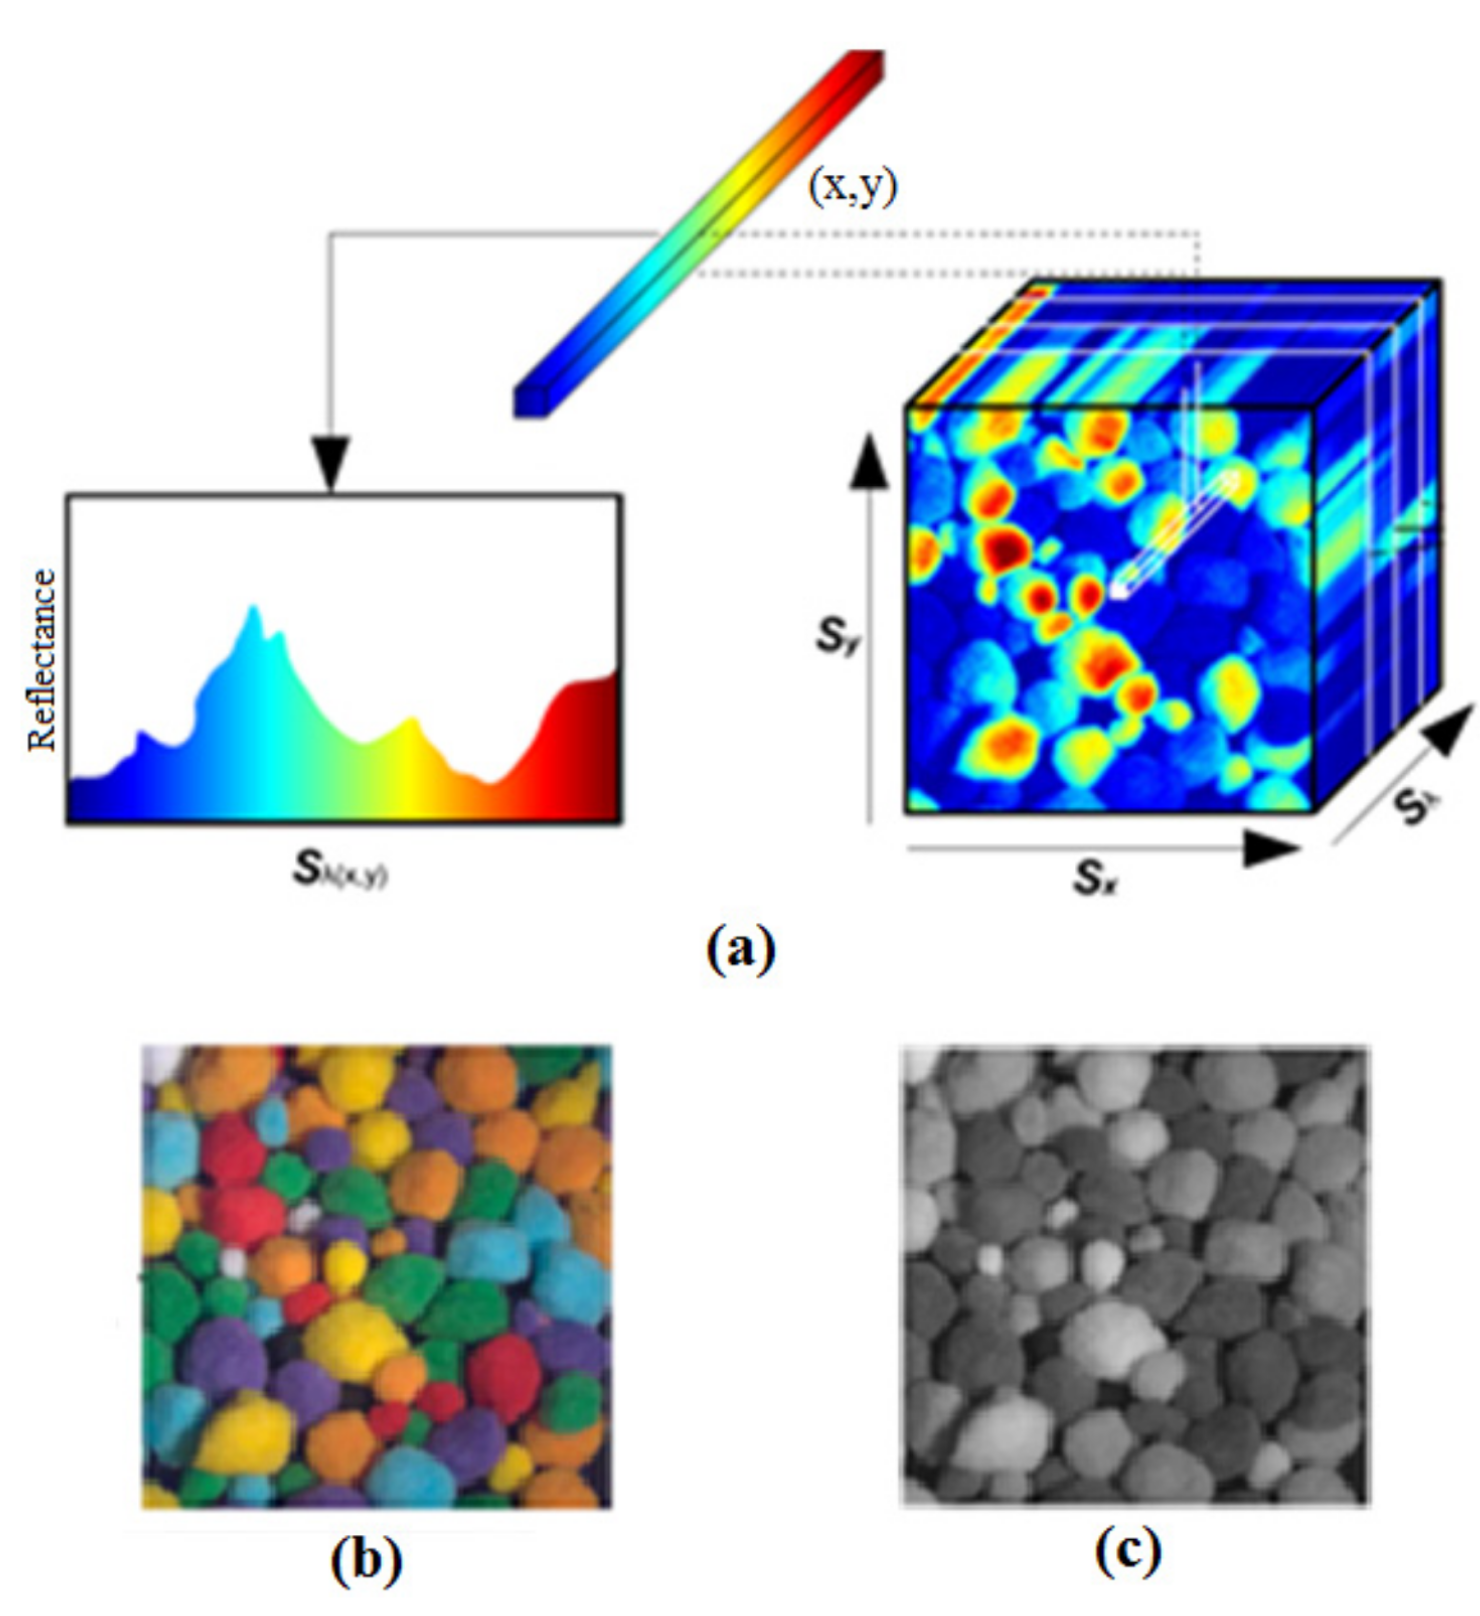
\includegraphics[width=1\linewidth]{figures/HSI_example.png}
            \captionsetup{labelformat=simple, labelsep=colon, font=scriptsize, labelfont={color=gray,bf}}
            \caption{(a) HSI Cube; (b) RGB Image; (c) Grayscale Image. \cite{khanModernTrendsHyperspectral2018}}
            \label{fig:khan-modern}
            \end{figure}
        \end{column}

        % Right column
        \begin{column}{0.62\textwidth}
            \begin{itemize}
                \item \textbf{Hyperspectral Images (HSIs)}: 
                \begin{itemize}
                    \item Capture spatial \& spectral properties.
                \end{itemize}
                \vspace{0.2cm}
                \item \textbf{Why Unsupervised Clustering?} 
                \begin{itemize}
                    \item Reveal hidden patterns
                    \item No need for labeled data
                \end{itemize}
                \vspace{0.2cm}
                \item \textbf{Challenges in HSIs:}
                \begin{itemize}
                    \item High dimensionality
                    \item Spectral/spatial variability
                    \item Noise \& distortions
                \end{itemize}
            \end{itemize}
        \end{column}
    \end{columns}
\end{frame}

%%% Local Variables:
%%% mode: latex
%%% TeX-master: "../topic-slide-main"
%%% End: